\section*{Partições}

\begin{frame}[fragile]{Partição}

    \metroset{block=fill}
    \begin{block}{Definição}
        Uma partição de um inteiro positivo $N$ corresponde a uma sequência de inteiros positivos
        $\{\ a_1, a_2, \ldots, a_k\ \}$ tais que $a_1 + a_2 + \ldots + a_k = N$.
    \end{block}

    \vspace{0.2in}

    Por exemplo, para $N$ = 5 há 7 partições distintas:
\[
        \{\ 5\ \}, \{\ 4, 1\ \}, \{\ 3, 2\ \}, \{\ 3, 1, 1\ \}, \{\ 2, 2, 1\ \}, \{\ 2, 1, 1, 1\ \}, \{\ 1, 1, 1, 1, 1\ \}
\]

Denotaremos $p(N)$ a cardinalidade do conjunto das partições de $N$. 

\end{frame}

\begin{frame}[fragile]{Partições e programação dinâmica}

Podemos interpretar o problema das partições como um problema do troco, onde as ``moedas'' seriam
os inteiros positivos de $1$ a $N$. Seja $\sigma(N, M)$ o número de partições de um inteiro positivo $N$ cujos elementos
são menores ou iguais a $M$. Os casos bases seriam:
\begin{enumerate}
    \item $\sigma(0, M) = 1$  (há uma única partição de zero: o conjunto vazio)
    \item $\sigma(N, 1) = 1$ (há uma única maneria de se particionar um número $N$ como somas de uns)
    \item $\sigma(N, 0) = 0$ (as partições deve ser compostas apenas por números positivos)
\end{enumerate}

As transições serão dadas por
\begin{itemize}
    \item $\sigma(N, M) = \sigma(N, M - 1)$,  se $M > N$ (não é possível escolher $M$: siga para a próxima moeda estritamente menor que $M$)
    \item $\sigma(N, M) = \sigma(N - M, M) + \sigma(N, M - 1)$,  se $M \leq N$ (há duas opções: escolher $M$ ou ignorá-lo)
\end{itemize}

\end{frame}

\begin{frame}[fragile]{Implementação de $p(N)$ em C++}

    \inputcode{cpp}{codes/dp.cpp}

\end{frame}

\begin{frame}[fragile]{Interpretação alternativa}

A implementação acima tem complexidade $O(N^2)$, o que permite computar $p(N)$ para valores de
$N$ menores ou iguais a aproximadamente $10^4$.

Na modelagem anteior $\sigma(N, M)$ significa ``o número de partições de $N$ que utilizam
valores menores ou iguais a $M$''. Podemos usar uma modelagem semelhante, mas como significado
ligeiramente diferente, o que será útil na definição de novos conceitos.

Seja $\rho(N, K)$ o número de partições de $N$ cujo maior elemento é igual a $K$. Os casos bases 
são
\begin{enumerate}
    \item $\rho(0, 0) = 1$ (existe uma única partição de zero com $K = 0: \{\ 0\ \}$)
    \item $\rho(N, K) = 0$, se $N \leq 0$ (as partições são definidas para inteiros positivos)
    \item $\rho(N, K) = 0$, se $K \leq 0$ (os elementos da partição devem ser inteiros positivos)
\end{enumerate}

\end{frame}

\begin{frame}[fragile]{Interpretação alternativa}

A transição seria
\[
        \rho(N, K) = \rho(N - K, K) + \rho(N - 1, K - 1)
\]

O primeiro termo da transição corresponde a tomar um termo $K$, que já garante a propriedade,
e tomar todas as possíveis partições de $N - K$ com a mesma restrição; a segunda parte 
corresponde as partições do antecessor $N - 1$ que tem elemento máximo $K - 1$: neste cenário,
basta escolher um dos elementos $K - 1$, somar o número $1$ a ele e obter uma partição de $N$ com elemento
máximo $K$.

Para verificar que esta transição conta todos as partições com máximo $K$ corretamente, veja que
a primeira parte contabiliza as partições que tem dois
ou mais termos iguais a $K$; já a segunda parte conta apenas as partições que tem exatamente
um elemento igual a $K$.

\end{frame}

\begin{frame}[fragile]{Implementação alternativa em C++}
    \inputsnippet{cpp}{1}{15}{codes/rho.cpp}
\end{frame}

\begin{frame}[fragile]{Implementação alternativa em C++}
    \inputsnippet{cpp}{17}{25}{codes/rho.cpp}
\end{frame}

\begin{frame}[fragile]{Partição conjugada}

É possível representar uma partição graficamente, e desta representação derivar uma importante
propriedade. Considere a partição $5 + 4 + 3 + 1$ de $13$. Estes números formam um matriz onde
cada coluna é formada por cada um destes números:
\begin{figure}[!h]
    \centering

    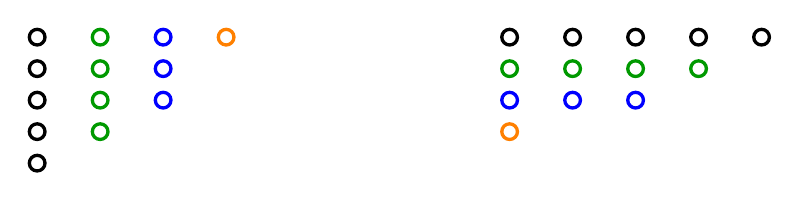
\begin{tikzpicture}
        \node[very thick,draw,circle,inner sep=2] at (0, 2) { };
        \node[very thick,draw,circle,inner sep=2] at (0, 1.6) { };
        \node[very thick,draw,circle,inner sep=2] at (0, 1.2) { };
        \node[very thick,draw,circle,inner sep=2] at (0, 0.8) { };
        \node[very thick,draw,circle,inner sep=2] at (0, 0.4) { };

        \node[very thick,draw,circle,inner sep=2,color=green!60!black] at (0.8, 2) { };
        \node[very thick,draw,circle,inner sep=2,color=green!60!black] at (0.8, 1.6) { };
        \node[very thick,draw,circle,inner sep=2,color=green!60!black] at (0.8, 1.2) { };
        \node[very thick,draw,circle,inner sep=2,color=green!60!black] at (0.8, 0.8) { };

        \node[very thick,draw,circle,inner sep=2,color=blue] at (1.6, 2) { };
        \node[very thick,draw,circle,inner sep=2,color=blue] at (1.6, 1.6) { };
        \node[very thick,draw,circle,inner sep=2,color=blue] at (1.6, 1.2) { };

        \node[very thick,draw,circle,inner sep=2,color=orange] at (2.4, 2) { };


        \node[very thick,draw,circle,inner sep=2] at (6, 2) { };
        \node[very thick,draw,circle,inner sep=2] at (6.8, 2) { };
        \node[very thick,draw,circle,inner sep=2] at (7.6, 2) { };
        \node[very thick,draw,circle,inner sep=2] at (8.4, 2) { };
        \node[very thick,draw,circle,inner sep=2] at (9.2, 2) { };

        \node[very thick,draw,circle,inner sep=2,color=green!60!black] at (6, 1.6) { };
        \node[very thick,draw,circle,inner sep=2,color=green!60!black] at (6.8, 1.6) { };
        \node[very thick,draw,circle,inner sep=2,color=green!60!black] at (7.6, 1.6) { };
        \node[very thick,draw,circle,inner sep=2,color=green!60!black] at (8.4, 1.6) { };

        \node[very thick,draw,circle,inner sep=2,color=blue] at (6, 1.2) { };
        \node[very thick,draw,circle,inner sep=2,color=blue] at (6.8, 1.2) { };
        \node[very thick,draw,circle,inner sep=2,color=blue] at (7.6, 1.2) { };

        \node[very thick,draw,circle,inner sep=2,color=orange] at (6, 0.8) { };

    \end{tikzpicture}
\end{figure}

As colunas da transposta desta matriz (lado direito da figura),
fornecem uma nova partição de $13$: $4 + 3 + 3 + 2 + 1$, a qual contém exatamente
$5$ elementos. A partição obtida através da matriz transposta de uma partição dada é denominada
a conjugada da partição.

\end{frame}

\begin{frame}[fragile]{Relação entre uma partição e sua conjugada}

    \metroset{block=fill}
    \begin{block}{Proposição}
        Seja $P$ uma particão cujo maior elemento é $K$. Então a conjugada $\bar{P}$ de $P$ contém exatamente $K$ elementos. Em outros termos,
        seja $q(N, K)$ o número de partições de $N$ que tem exatamente $K$ elementos. Então
        \[
            \rho(N, K) = q(N, K)
        \]
    \end{block}

\end{frame}
\begin{frame}[fragile]{Partições autoconjugadas}

    \metroset{block=fill}
    \begin{block}{Definição}
        Uma partição é denominada autoconjugada se ela é igual a sua conjugada. 
    \end{block}

    \vspace{0.2in}

    Por exemplo, a partição $3 + 2 + 1$ de $6$ é autoconjugada: veja sua matriz abaixo

    \begin{figure}[!h]
        \centering

        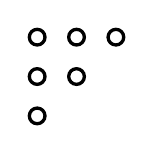
\begin{tikzpicture}
            \node[very thick,draw,circle,inner sep=2] at (0, 2) { };
            \node[very thick,draw,circle,inner sep=2] at (0, 1.5) { };
            \node[very thick,draw,circle,inner sep=2] at (0, 1.0) { };

            \node[very thick,draw,circle,inner sep=2] at (0.5, 2) { };
            \node[very thick,draw,circle,inner sep=2] at (0.5, 1.5) { };

            \node[very thick,draw,circle,inner sep=2] at (1.0, 2) { };
        \end{tikzpicture}
    \end{figure}

\end{frame}

\begin{frame}[fragile]{Propriedade das partições autoconjugadas}

As partições autoconjugadas também tem uma importante propriedade. Considere a partição
$6 + 5 + 4 + 4 + 2 + 1$ de $22$ e observe a separação em níveis feitas por cores:

    \begin{figure}[!h]
        \centering

        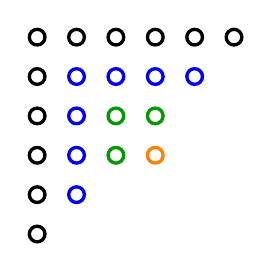
\begin{tikzpicture}
            \node[very thick,draw,circle,inner sep=2] at (0, 2.5) { };
            \node[very thick,draw,circle,inner sep=2] at (0, 2.0) { };
            \node[very thick,draw,circle,inner sep=2] at (0, 1.5) { };
            \node[very thick,draw,circle,inner sep=2] at (0, 1.0) { };
            \node[very thick,draw,circle,inner sep=2] at (0, 0.5) { };
            \node[very thick,draw,circle,inner sep=2] at (0, 0) { };

            \node[very thick,draw,circle,inner sep=2] at (0.5, 2.5) { };
            \node[very thick,draw,circle,inner sep=2] at (1, 2.5) { };
            \node[very thick,draw,circle,inner sep=2] at (1.5, 2.5) { };
            \node[very thick,draw,circle,inner sep=2] at (2, 2.5) { };
            \node[very thick,draw,circle,inner sep=2] at (2.5, 2.5) { };

            \node[very thick,draw,circle,inner sep=2,color=blue] at (0.5, 2.0) { };
            \node[very thick,draw,circle,inner sep=2,color=blue] at (0.5, 1.5) { };
            \node[very thick,draw,circle,inner sep=2,color=blue] at (0.5, 1.0) { };
            \node[very thick,draw,circle,inner sep=2,color=blue] at (0.5, 0.5) { };

            \node[very thick,draw,circle,inner sep=2,color=blue] at (2.0, 2.0) { };
            \node[very thick,draw,circle,inner sep=2,color=blue] at (1.0, 2.0) { };
            \node[very thick,draw,circle,inner sep=2,color=blue] at (1.5, 2.0) { };

            \node[very thick,draw,circle,inner sep=2,color=green!60!black] at (1.0, 1.5) { };
            \node[very thick,draw,circle,inner sep=2,color=green!60!black] at (1.0, 1.0) { };
            \node[very thick,draw,circle,inner sep=2,color=green!60!black] at (1.5, 1.5) { };

            \node[very thick,draw,circle,inner sep=2,color=orange] at (1.5, 1.0) { };
        \end{tikzpicture}
    \end{figure}

Esta é uma permutação autoconjugada. A soma dos elementos de cada nível gera a partição
$11 + 7 + 3 + 1$, uma partição de $22$ que contém apenas números ímpares distintos. Isto
nos leva a outro importante resultado: o número de partições autoconjugadas de $N$ é igual ao
número de partições de $N$ que contém apenas fatores ímpares distintos.

\end{frame}

\begin{frame}[fragile]{Partições e Análise Combinatória}

    \metroset{block=fill}
    \begin{block}{Proposição}

        Seja $q(N, K)$ o número de partições de $N$ que tem exatamente $K$ elementos. Então o 
        número de maneiras de se distribuir $N$ objetos idênticos, em $K$ caixas idênticas, sem que
        nenhuma das caixas fique vazia, é igual a $q(N, K)$.
    \end{block}

\end{frame}


